
% --------------------------------------------------------------
\begin{chapter}{Decision Making with Complex Models \label{Chap:optimisation}}

In many settings, a model --- of any complexity --- can be constructed and then deployed to aid decision making. Bayesian decision theory gives us a mature and coherent framework for combining the decision maker's prior beliefs and preferences with a model, including complex stochastic simulators. Recall that if the decision maker represents their preferences for a decision $\bx \in \mathcal{X}$ by a utility function $u(\bx, \btheta)$, they represent their beliefs about all uncertain quantities by a prior distribution $\btheta \sim \pi(\btheta)$ and the expected utility of a decision is $U(\bx) = \E_{\btheta} \{ u(\bx, \btheta) \}$, then the optimal decision is defined as
\begin{equation}
 \bx^{*} = \argmax_{\bx \in \mathcal{X}} U(\bx).
\end{equation}
Prior beliefs, $\pi(\btheta)$, should be replaced by posterior beliefs, $\pi(\btheta | \by)$, when relevant data, $\by$, are available.

Once the decision problem has been defined by an appropriate belief structure as above, the decision problem is reduced to an optimisation problem. Although the problem is `reduced', the enormous literature on mathematical and numerical optimisation should serve as a warning that the reduced problem is usually far from trivial. The difficulty is amplified when the utility function is expensive to compute, is noisy and no gradient information is available. This can be because $U(\bx)$ itself is expensive to compute or depends on the output of one or more computationally expensive simulators \citep{Williamson2012}. Both situations are commonly seen in Bayesian design of experiments or subjective Bayesian analyses when viewing a large collection of samples from the posterior distribution with negligible autocorrelation as the output of a computationally expensive simulation (e.g. a long run of an MCMC scheme) \citep{Ryan2016, Vernon2022bayes}. Our analysis will use relatively simple utility functions; however, the utility function itself depends on output of the Athena model. Therefore, $U(\bx)$ will be expensive to compute.

We now discuss the various types of optimisation problem that arise and methods to solve them.

\section{Discrete problems}
\subsection{Small, discrete problems}
Suppose that there is no obvious structure to the decision problem, or the number of decisions that can be taken is small. In a wind farm setting this could be considering where to place the farm from a small number of candidate locations. If we consider $n$ locations $\mathcal{X} = \{ \bx_1, \bx_2, \ldots \bx_n \}$ then the best we can do is just evaluate $U(\bx_i)$ for each $i$.

When the decision is made under uncertainty, the simplest approach is to use a Monte Carlo approximation of $U(\bx_i)$. If evaluating $u(\bx, \btheta)$ is expensive because, for example, the utility of a decision depends on the result of a complex computer model, we may wish to construct an emulator for $u(\cdot)$ as a function of uncertain quantities $\bm{\btheta}$ and decision variables $\bx$. That is, construct a surrogate, $\hat{u}(\bx, \btheta)$ and propagate beliefs $\pi(\bm{\btheta})$ through $\hat{u}(\bx, \btheta)$. This is precisely what \citet{Oakley2009} does, and achieves a tractable approximation to $U(\bx_i)$ via a GP emulator.

Another option for discrete problems is Thompson Sampling (TS). If the number of simulator evaluations we can make is limited, we may want to carefully allocate simulator runs in a sequential manner. TS originated in two-armed bandit problems \citep{Thompson1933} and has enjoyed recent success in multi-armed bandit problems since it is simple but effective \citep{Scott2010, Chapelle2011}. The approach to solving a multi-armed bandit problem via TS is to randomly allocate simulator runs one-by-one to a pre-defined set of inputs. This sequential allocation balances exploitation of inputs which are likely to give rise to good solutions whilst acknowledging that simulator outputs are uncertain, thus the uncertainty should be resolved via exploring the decision space.

When the decision set is small and discrete we may be able to phrase the problem as a multi-armed bandit problem. For example, suppose we have $U(\bx) = \p (A(\bx) > A^{*}) = \E \{\mathbb{I}(A(\bx) > A^{*}) \} $, and we have a small number of distinct values of $\bx$ corresponding to discrete decisions. These decisions, for example, could be a small collection of different locations at which the wind farm could be constructed. Running the Athena simulator at a candidate decision $\bx$ will give us an availability which is either above $A^{*}$ or not. After $n$ simulator runs at different values of $\bx$ (with some replication) we are able to obtain probabalistic estimates for each $U(\bx)$. Since, in this example, $U(\bx)$ is a probability, a Beta distribution would be an appropriate probabalistic representation of $U(\bx)$. The Beta prior distribution allows us to estimate $U(\bx) = P(A(\bx) > A^{*})$ via conjugate Bayesian inference. If, prior to running any simulations, $U(\bx_i) \sim Beta(a_{i,0}, b_{i,0})$, then once we have evaluated $u(\cdot)$ $n_i > 0$ times at simulator input $\bx_i$, the posterior distribution will be $Beta(a_{i,n_i}, b_{i, n_i})$ where
\begin{align}
 a_{i, n_i} & = a_{i, 0} + \sum_{j = 1}^{n_i} \mathbb{I} \left\{ A(\bx_i)_j > A^{*} \right\} \nonumber\\
 b_{i, n_i} & = b_{i, 0} + \sum_{j = 1}^{n_i} \mathbb{I} \left\{ A(\bx_i)_j \leq A^{*} \right\}\nonumber
\end{align}
where $A(\bx_i)_j$ is the $j$th draw of $A(\bx_i)$. If $n_i = 0$ then the prior cannot be updated; our prior beliefs will be the representation of our knowledge. TS tells us to next run the simulator at the input which maximises
\begin{equation}
 \bx_j = \argmax_{i \in \{1, 2, \ldots, n \} } \tilde{U}(\bx_i)
\end{equation}
where $\tilde{U}(\bx_i)$ are independent, random draws of $U(\bx_i) \sim Beta(a_{i, n_i}, b_{i, n_i})$. The random draws induce an exploration-exploitation trade-off. Randomness allows for exploration as it accounts for uncertainty about the $U(\bx_i)$. Exploitation comes into play though the posterior distributions. If the posterior density of $U(\bx_i)$ is concentrated about large values of $U(\bx_i)$, then the probability that the simulator is run at $\bx_i$ will increase. We can also allow for exploitation of prior knowledge via the prior; $a_{i,0} \in \N$ and $b_{i,0} \in \N$ can be interpreted as \textit{a priori} counts for the events $A(\bx_i) > A^{*}$ and $A(\bx_i) \leq A^{*}$ respectively. This approach can be extended to continuous problems, which is considered later.
\subsection{Structured, discrete problems}
Some decision problems are discrete in nature but far too complex for a brute force computation. The lack of smoothness in such problems makes emulation difficult. In some situations we cannot solve the decision problem exactly because of these computational constraints. We must settle for the best solution possible in the time available.

In complex, discrete problems the expected utility surface can be very rough with respect to the decision space. A well-known example of such a problem is the Travelling Salesman Problem (TSP) in which a salesman aims to visit a fixed set of locations, by traversing the edges of a graph, in such a way that costs are minimised. Phrasing as a decision problem, if $\ell(\bx)$ is the cost of the path taken by the salesman, we would take $U(\bx) \propto \ell(\bx)$. In this case, a small change in the path might lead to a not so small change in $U(\bx)$, that is, if $||\bx - \bx'||$ is small, there is no reason to believe that $||U(\bx) - U(\bx')||$ is also small \citep{Gutin2007}.

A mathematically simple approach is a random search. Take a random sample $\mathcal{X}_0 = \{ \bx_1, \bx_2, \ldots, \bx_n\}$ from $\mathcal{X}$. Then an approximation to the optimal decision is $\hat{\bx} = \argmax_{\bx \in X_0} U(\bx)$. If the computational budget is large enough, we would find $\bx^{*}$. In practice, this can be a big ``if''. Convergence to the optimum requires many evaluations of $U(\bx)$ when knowledge of $U(\bx)$ is ignored \citep{Kan1989}. Beyond this, random search serves as a benchmark: if random search does better than a seemingly more intelligent method, then perhaps the method is not as intelligent as first thought.

An adaptation of (purely) random search is stochastic optimisation. A common example is simulated annealing (SA), which is inspired by the process of annealing in metallurgy \citep{Kirkpatrick1983, Schneider2006}. SA is one of many stochastic optimisers, and can perform well when the decision surface is very rough. Given a candidate solution $\bx'$ and a `current' solution $\bx_t$ we take $\bx_{t+1} = X_{t+1}$ where $X_{t+1}$ is a random variable which takes the value $\bx'$ with probability $\alpha( \bx' \mid \bx_{t}, t)$ and $\bx_t$ otherwise. The candidate decision will typically be a modified version of $\bx_t$. If the decision space is a subset of $\R^k$, we might form $\bx'$ by setting $\bx' = \bx_t + \mathcal{N}(0, \sigma^2I_k)$ where $\sigma^2$ is a tuning parameter. For discrete problems, we may randomly change individual aspects of $\bx$ to construct $\bx'$. For example, if $\bx$ is a vector of binary values, we may set $x_i' = 1 - x_i$ for some randomly chosen $i$. Typically $\alpha(\bx' \mid \bx_{t}, t)$ should favour $\bx'$ for small values of $t$, corresponding to exploratory behaviour in early stages, but as $t$ increases, $\alpha(\bx' \mid \bx_{t}, t)$ should begin to favour $\argmax \{U(\bx_t), U(\bx')\}$, corresponding to increasing levels of exploitation. A common form for alpha is
\begin{equation}
 \alpha(\bx' \mid \bx_{t}, t) = \min \left\{ \exp\left[-\frac{U(\bx_t) - U(\bx')}{Kt}\right], 1\right\}
\end{equation}
where $K$ is a tuning parameter which controls the rate of the annealing schedule. SA can be thought of as a random walk which is designed to maximise $U(\bx)$. SA cannot not really exploit any structure in $U(\bx)$ (and is designed for situations where $U(\bx)$ has little structure) thus may require many evaluations of $U(\bx)$ to find a close-to-optimal solution. Within the emulation literature, SA has been successful in providing optimal Latin hypercube designs \citep{Morris1995, Pholdee2015}.

A discrete structure which can be exploited through surrogate modelling is permutations. Consider a set of tasks $\{T_1, T_2, \ldots, T_J\}$. If there are $J$ tasks to complete, then $J!$ permutations need to be considered. For moderately small $J$, $J!$ can be very large and grows incredibly quickly ($3! = 6$, $6! = 720$, $10! = 3628800$). Computing $U(\bx)$ for all possible $\bx$ can quickly become very time consuming, especially if $U(\cdot)$ is expensive. To alleviate this, \citet{Wilson2018} use a surrogate inspired by the Benter model \citep{Benter1994} to efficiently find an approximate solution to their permutation-based problem.
\subsection{Continuous problems}
If the decision space is continuous, e.g. $\bx \in \mathcal{X} \subseteq \mathbb{R}^n$ and we have relatively easy access to $U(\bx)$, we can use standard optimisation routines like \verb|optim| in \verb|R|. Continuity allows us to embrace calculus when we have easy access to $U(\bx)$. By `easy access' we mean that $U(\bx)$ is available in closed form, or we have access to highly accurate approximations such as Monte Carlo estimates with negligible standard errors.

However, evaluation of $U$ might be sufficiently difficult to make standard optimisation methods cumbersome. When evaluations of $U(\bx)$ are limited for computational or financial reasons, such as running simulations in a pay-per-usage cloud server, requires collection of primary data, human interaction or is otherwise computationally expensive, we may use a surrogate to reduce optimisation costs \citep{Tresidder2012, Astudillo2020}.

Broadly, we can use a surrogate to perform optimisation in two ways. The first way is to construct a one-shot design (via, for example, a Latin Hypercube) to construct an emulator or surrogate $\hat{U}(\bx)$. Maximising $\hat{U}(\bx)$ will provide an approximate solution to the decision problem. For examples of this approach see \citep{Wilson2018, Overstall2017}. The second way is to view optimisation as a sequential design problem, which we explore in the next section.

\section{Bayesian optimisation}
Instead of directly maximising the surrogate, $\hat{U}(\bx)$, it may be advantageous to use our knowledge of $U(\bx)$, expressed as a posterior distribution, to guide us towards values of $\bx$ which are likely to improve on the largest value of $U(\bx)$ seen so far. This is essentially what numerical optimisation does. A standard Newton-Raphson scheme uses the gradient of $U(\bx)$ to speculate where a larger value of $U(\bx)$ may lie. Newton-Raphson uses only local knowledge of $U(\bx)$. Gaussian processes have a global \emph{and} a local understanding of $U(\cdot)$, this can be leveraged.

An approach known as \textit{Bayesian Optimisation} (BayesOpt) uses global and local knowledge, expressed via a posterior distribution, to maximise $U(\bx)$. The core idea behind BayesOpt is to construct an emulator for $U(\bx)$ and use this to guide our search towards $\bx^{*}$ \citep{Frazier2018}. Although much of the BayesOpt language is plagued by machine learning jargon, BayesOpt is actually a form of sequential design. BayesOpt has been found to be useful in a variety of optimisation problems where $U(\bx)$ has some, or even all, of the following properties
\begin{itemize}
 \item $U(\bx)$ is costly to evaluate
 \item $U(\bx)$ possess multiple local optima
 \item derivatives, $\frac{\partial U(\bx)}{\partial x_i}$, are not available
 \item $U(\bx)$ is thought to be quite smooth
 \item $\bx$ is of not too large dimension (less than about $20$).
\end{itemize}
The Athena simulator possesses many of these properties. In particular, we know that it is expensive to evaluate, has no closed form gradient expressions and we think that many quantities output by Athena are reasonably smooth. We do not know how many local optima Athena has, and that may depend on which input-output combinations are used for optimisation.

BayesOpt is a promising framework for solving decision problems with the Athena simulator. Not all of these properties have to hold for BayesOpt to be a suitable approach. For example, knowledge about maxima or gradient information can be leveraged \citep{Wu2017, Nguyen2020}. The key properties are that $U(\bx)$ is costly and smooth; if it were not, other methods could be more appropriate. A common application of BayesOpt is tuning machine learning models \citep{Joy2016, Snoek2012}. BayesOpt dates back to at least \citet{Mockus1975} who used (Bayesian) linear models as the surrogate. The modern incarnation of BayesOpt has stemmed from \citet{Jones1998} who popularised the use of more flexible covariance structures (for example, the squared exponential) within BayesOpt. BayesOpt can be viewed as a sequential design strategy for global maximisation (or minimisation) of expensive black-box functions, see \citet{Frazier2018} for an overview.

We will take a diversion from the Athena simulator and decision making to consider BayesOpt for arbitrary functions, rather than utility functions. Suppose we observe $y(\bx) = f(\bx) + \varepsilon(\bx)$ where $f(\cdot)$ is the function to be maximised and $\varepsilon(\bx)$ is (possibly input dependent) noise, which is assumed to be independent of other error terms, Gaussian and additive. We start by specifying the joint model for $(\by^T, f(\bx))$ and use the conditional Normal equations to provide the posterior moments for $f(\bx) \mid \by$
\begin{align}
 \begin{pmatrix} \by \\ f(\bx) \end{pmatrix}
  &\sim \mathcal{N} \left\{
  \begin{pmatrix} \mu(X) \\ \mu(\bx) \end{pmatrix}, \begin{pmatrix} \Sigma_{X, X} & \Sigma_{X, \bx} \\ \Sigma_{\bx, X} & \sigma^2 \end{pmatrix}
  \right\} \\
  f(\bx) \mid \by &\sim \mathcal{N}(m^{*}(\bx), v^{*}(\bx) )
\end{align}
where $X$ are the locations at which the simulator has been run, $\mu(\cdot)$ is the prior mean function, $\Sigma_{X, X} = \var\{\by\}$, $\sigma^2 = \var\{f(\bx)\}$, $\Sigma_{X, \bx} = \Sigma_{\bx, X}^T = \cov\{y(X), f(\bx)\}$ and $m^{*}(\bx)$ and $v^{*}(\bx)$ are the posterior mean and variance, as found by the multivariate Normal equations; \cref{Eq:MV1} and \cref{Eq:MV2}.
\subsection{Acquisition functions}
Once an emulator has been fit to a small collection of initialisation runs, we can start to use the emulator to make intelligent choices about where to next run the simulator so that $f(\bx)$ can be efficiently optimised. The device that allows us to make decisions about where to next evaluate $f(\bx)$ is an \textit{acquisition function}. The acquisition function is a function of $\bx$ and the posterior distribution on $f(\bx)$ which aims to find large values of $f(\bx)$. We introduce new notation for the posterior on $f(\cdot)$ which is better suited to online learning/sequential inference. Suppose we have observed $n$ runs of the simulator: $\mathcal{D}_n = \{(\bx_1, y_1), (\bx_2, y_2), \ldots, (\bx_n, y_n)\}$. The `time $n$' posterior for $f(\cdot)$ (after observing $n$ runs) is denoted $\pi_n(f(\cdot) \mid \mathcal{D}_n, \Theta_n)$ where $\Theta_n$ are the time $n$ GP hyperparameters. We will abuse notation here and use $\pi_n(f(\cdot))$ as shorthand for $\pi_n(f(\cdot) \mid \mathcal{D}_n, \Theta_n)$. We then define, using the dummy variable $y = f(\bx)$,
\begin{equation}
 \E_n\{g(f(\bx))\} = \int_{-\infty}^{\infty} g(v) \pi_n(y) \,\dd v
\end{equation}
as the expected value of $g(f(\bx))$ with respect to $\pi_n(f(\bx))$, for any function $g(\cdot)$ at a known input $\bx$. This additional notation is useful since acquisition functions can often be expressed as expectations of a function of $f(\bx)$, having observed $n$ simulator runs. This means that many acquisition functions have a decision theoretic justification because they are expressed as expectations of utility functions. Having observed $n$ simulator runs, and \correction{assuming that $\E_n(f(\bx))$ has a single global optimum,} the time $n$ optimal solution is
\begin{equation}
 \hat{\bx}_n = \argmax_{\bx \in X_n} \E_n \{ f(\bx) \} \label{Eq:best-so-far}
\end{equation}
where $X_n$ is the set of input configurations at which the simulator has been run. When $f(\cdot)$ is a deterministic function, $\hat{\bx}$ corresponds to the input which, so far, has given the largest function output. This is precisely the value that would be used under any other optimiser. When $f(\cdot)$ is observed with noise, \cref{Eq:best-so-far} is the value of $\bx$ leading to the largest posterior mean. This follows naturally from Bayesian decision theory. We now introduce some more notation to allow a fluent discussion of common acquisition functions. Let $y^{*}_n = \E_n \{ f(\hat{\bx}_n) \}$, let $\mu_n(\bx) = \E_n \{ f(\bx) \}$ and let $\sigma^2_n(\bx) = \var_n\{ f(\bx) \} = \E_n \left\{ \left[ f(\bx) - \mu_n(\bx) \right]^2 \right\}$, where $\bx \in \mathcal{X}$ is any valid input.
\subsubsection{Probability of improvement}
The first acquisition function we encounter is the probability of improvement (PI) denoted $\alpha_{PI}$. Consider the following utility function over possible values of $f(\bx)$:
\begin{equation}
 \tilde{\alpha}_{PI}(\bx) =
 \begin{cases}
  1,& f(\bx) > y^{*}_n \\
  0,& f(\bx) \leq y^{*}_n
 \end{cases}
\end{equation}
that is, an indicator utility function returning $1$ when we improve upon $y_n^{*}$ and returning $0$ when there is no improvement. This expresses the belief that all improvements, regardless of size, are equally preferable. We then have $\alpha_{PI}(\bx) = \E_n \{ \tilde{\alpha}_{PI}(\bx) \}$. The expectation of an indicator function is the probability of the event in question, thus we have
\begin{align}
 \alpha_{PI}(\bx) &= \p(f(\bx) > y^{*}_n)\label{Eq:prob-imp}\\
  &= \Phi\left(\frac{ \mu_{n}(\bx) - y^{*}_n }{\sigma_{n}(\bx)}\right). \label{Eq:prob-imp-gp}
\end{align}
Regardless of the chosen statistical model, \Cref{Eq:prob-imp} provides the probability of improvement; this will be available in closed form for a large class of statistical models. If the closed form is not available, a highly accurate approximation is likely to be built into popular scientific computing libraries. Under GP assumptions, the probability of improvement can be expressed as \Cref{Eq:prob-imp-gp} which, technically, is not tractable but good approximations are widely available, for example, \texttt{pnorm()} from \texttt{R}.
\subsubsection{Expected improvement}
A criticism of PI as an acquisition function is that PI sees all possible improvements as equally good, regardless of the magnitude of the improvement. Suppose that $y^{*}_n = 0$ and further suppose $f(\bx_1) \sim N(0, 1)$ and $f(\bx_2) \sim N(0, 10)$. We see that $\alpha_{PI}(\bx_1) = \alpha_{PI}(\bx_2) = 0.5$, therefore, this BayesOpt scheme views $\bx_1$ and $\bx_2$ as equally promising. However, the potential gains under $\bx_2$ are much larger than the potential gains under $\bx_1$. The nature of PI can be investigated via partial derivatives. We see that $\frac{\partial \alpha_{PI}(\bx)}{\partial \mu_n(\bx)} = \frac{1}{\sigma_n(\bx)}\phi\left( \frac{\mu_n(\bx) - y^{*}_n}{\sigma_n(\bx)} \right) > 0$ thus, increasing $\mu_n(\bx)$ increases $\alpha_{PI}(\bx)$. Therefore, inputs corresponding to function values with large predictive means are favoured. However, $\frac{\partial \alpha_{PI}(\bx)}{\partial \sigma_n(\bx)} = -\frac{\mu_n(\bx) - y^{*}_n}{\sigma_n(\bx)^2}\phi\left( \frac{\mu_n(\bx) - y^{*}_n}{\sigma_n(\bx)} \right)$. The sign of this expression depends on $\mu_n(\bx) - y^{*}_n$. In particular, $\text{sign}\, \left\{\frac{\partial \alpha_{PI}(\bx)}{\partial \sigma_n(\bx)}\right\} = \text{sign}\,\{y^{*}_n - \mu_n(\bx)\}$, therefore increasing $\sigma_n(\bx)$ increases $\alpha_{PI}(\bx)$ whenever $\mu_n(\bx) < y^{*}_n$ but decreases $\alpha_{PI}(\bx)$ when $\mu_n(\bx) > y^{*}(\bx)$ and $\alpha_{PI}(\bx) = 0.5$ when $\mu_n(\bx) = y^{*}(\bx)$. This means that we tend not to explore areas in which $f(\bx)$ is uncertain but has moderately large values of $\mu_n(\bx)$. The way PI deals with uncertainty is unsatisfactory; if $f(\bx)$ is thought to be large but $\var\{f(\bx)\}$ is also large, this is a region of the input space that should be explored further as the potential gains are large. This criticism can be boiled down to the fact that PI does not consider how large the potential change in $y_n^{*}$ is.

This motivates \textit{Expected Improvement} (EI) which gives a reward proportional to the improvement. First we define the improvement by
\begin{equation}
 \tilde{\alpha}_{EI}(\bx) = \max\{0, f(\bx)-y^{*}_n\}.
\end{equation}
This is intuitive: if $f(\bx) \leq y^{*}_n$ our best value has not improved. But if $f(\bx) > y^{*}_n$ then we have improved our current best value of $f(\cdot)$ by $f(\bx) - y^{*}_n$. Now since $f(\bx)$ is unknown, we integrate out $f(\bx)$, which has density $\pi_n(f(\bx))$, and thus the EI is
\begin{equation}
 \alpha_{EI}(\bx) = \E_n \{ \tilde{\alpha}_{EI}(\bx) \}.
\end{equation}
Under standard GP assumptions, we have an analytic expression for EI in terms of the Normal CDF and PDF. We aim to maximise $f(\cdot)$, so the acquisition function can be expressed as \citep{Pourmohamad2021}:
\begin{equation}
 \alpha_{EI}(\bx) = \begin{cases}
           \sigma_n(\bx)\phi\left(\frac{\mu_n(\bx)-y^{*}_n}{\sigma_n(\bx)}\right) + (\mu_n(\bx) - y_n^{*})\Phi\left(\frac{\mu_n(\bx)-y^{*}_n}{\sigma_n(\bx)}\right),&  \sigma_n(\bx) > 0 \\
           0, &  \sigma_n(\bx) = 0
           \end{cases}. \label{Eq:EI-defn}
\end{equation}
The EI is $0$ when $\sigma_n(\bx) = 0$ because $\sigma_n(\bx) = 0$ if, and only if, we know the value of $f(\bx)$ precisely. $f(\bx)$ will either be $y_n^{*}$ or be smaller than $y_n^{*}$ and hence offers no improvement. Although EI was constructed with deterministic problems in mind, it generalises naturally to the stochastic case. The exploitation-exploration trade-off under EI is fairly transparent. The first term of EI is multiplied by $\sigma_n(\bx)$, thus large uncertainty leads to larger values of $\alpha_{EI}$. The second term is multiplied by $\mu_n(\bx) - y_n^{*}$, thus large mean predictions typically increase EI. Applying basic calculus rules to \cref{Eq:EI-defn} leads to $\frac{\partial \alpha_{EI}(\bx)}{\partial \mu_n(\bx)} = \Phi \left( \frac{\mu_n(\bx) - y^{*}_n}{\sigma_n(\bx)} \right) > 0$ and $\frac{\partial \alpha_{EI}(\bx)}{\partial \sigma_n(\bx)} = \phi \left( \frac{\mu_n(\bx) - y^{*}_n}{\sigma_n(\bx)} \right) > 0$, thus EI increases with both $\mu_n(\bx)$ and $\sigma_n(\bx)$. That is, for fixed $\mu_n(\bx)$, a more uncertain value is a preferred input to run the simulator at, whilst if $\sigma_n(\bx)$ is fixed we will run the simulator at the input with greatest predicted value.

There are many extensions to EI which take into account problem structure. Examples include optimisation under unknown (black-box) constraints which learns the optimum input/output and the constraints \citep{Gramacy2010}. Batch (or ``multi-point'') EI runs the simulator at multiple, promising solutions simultaneously to take advantage of abundant cores in a parallel computing setting \citep{Marmin2015, Diessner2022}.
\subsubsection{Upper credible bound}
Another common acquisition function is the upper credible bound, or upper confidence bound, depending on the chosen interpretation of probability \citep{Srinivas2009}. Both can be abbreviated to UCB.
The UCB acquisition function is, under a GP model for $f(\cdot)$,
\begin{equation}
 \alpha_{UCB}(\bx \mid \nu_n) = \mu_n(\bx) + \nu_n \sigma_n(\bx). \label{Eq:ucb}
\end{equation}
where $\nu_n > 0$ are a sequence of tuning parameters controlling the exploration-exploitation trade-off. UCB was proposed with maximisation in mind but if minimisation is required we can use the lower credible/confidence bound instead.
\begin{equation}
 \alpha_{LCB}(\bx \mid \nu_n) = \mu_n(\bx) - \nu_n \sigma_n(\bx).
\end{equation}
For many statistical models, \cref{Eq:ucb} is an upper credible/confidence bound. We can adjust $\nu_n$ as appropriate. This means that in principle, UCB gives a tractable acquisition function for $f(\bx)$, whenever the chosen emulator has a tractable mean and variance. If $f(\bx)$ is not modelled \textit{a priori} by a GP, the expected improvement would likely be intractable.
 If desired, we can take $\nu_n = \nu$ for all $n$. Now since UCB is a linear combination of the posterior mean and standard deviation, the exploration-exploitation trade-off is transparent. Increasing $\mu_n(\bx)$ or $\sigma_n(\bx)$ whilst the other remains fixed clearly increases $\alpha_{UCB}(\bx \mid \nu_n)$. The trade off is controlled by $\nu_n$. Setting $\nu_n = 0$ leads to a pure exploitation regime: maximise the posterior mean. Letting $\nu_n \to \infty$ leads to picking the point with highest uncertainty, which is essentially ALM (\cref{Eq:std-alm}). Choosing a moderate value of $\nu_n$ leads to an exploration-exploitation compromise. The UCB acquisition function is sometimes called an `optimistic' approach; we are choosing $\bx_{n+1}$ based on an upper estimate for $f(\bx_{n+1})$.

Although not immediately obvious, we can actually write $\alpha_{UCB}(\bx)$ as the expected value of a random variable. \citet{JamesWilson2018} show that
\begin{equation}
 \alpha_{UCB}(\bx \mid \nu_n) = \int_{-\infty}^{\infty}\frac{\left( \mu_n(\bx) + |f(\bx) - \mu_n(\bx)| \right)}{\sqrt{2 \pi \tilde{\sigma}^2}} \exp \left\{ -\frac{(f(\bx) - \mu_n(\bx))^2}{2 \tilde{\sigma}^2} \right\} \dd f(\bx)
\end{equation}
where $\tilde{\sigma} = \sqrt{2 \pi \nu_n} \sigma$. This means that the UCB acquisition can be written as the following expectation
\begin{equation}
  \alpha_{UCB}(\bx \mid \nu_n) =\E_{\tilde{y}} \{\tilde{y}\}
\end{equation}
where $\tilde{y} \sim tr\mathcal{N}(\mu(\bx), \tilde{\sigma}^2(\bx); \mu(\bx), \infty)$ where $tr\mathcal{N}(m, s^2; a, b)$ denotes a Normal distribution truncated below at $a$, above at $b$ and the distribution to be truncated is $\mathcal{N}(m ,s^2)$. Therefore $\alpha_{UCB}(\bx)$ can be interpreted, in a decision theoretic context, as the expected value of a linearly transformed and truncated version of $f(\bx)$. This is quite difficult to interpret but this representation of UCB was constructed with computation, not interpretation, in mind \citep{Wilson2017}.
\subsubsection{Thompson sampling}
There is a stochastic approach to BayesOpt; Thompson sampling (TS). By stochastic, we mean that the acquisition function is randomly generated. Whether the simulator is stochastic or deterministic is not critical in this context. The idea behind TS is to draw a random function $g(\cdot) \sim \pi_n(f(\cdot))$ and then use $g(\cdot)$ as an acquisition function. The next point at which to run $f(\bx)$ is then given by the maximiser of this drawn function:
\begin{equation}
 \bx_{n+1} = \argmax_{\bx \in \calX} g(\bx).
\end{equation}
We discussed earlier that TS is useful in multi-armed bandit problems. With a GP framework, for problems defined over a continuous domain, a full draw from $\pi_n(f(\cdot))$ is impossible; this in an object of infinite dimension. The best we can do is draw $g(\tilde{X})$ from $\pi_n(f(\tilde{X}))$ where $\tilde{X}$ is a large, but finite, collection of inputs. This can cause problems in high dimensional settings due to the curse of dimensionality; $\tilde{X}$ will almost always be sparse within the input space. This can be combated by `extending' the realised function by adding rows to the lower Cholesky decomposition of $\var_n \{ f(\tilde{X}) \}$. Algorithms for extending the Cholesky decomposition are discussed by \citet{Higham2009}. This means that maximising $g(\cdot)$ when the decision space is either continuous or large and discrete is difficult. However, the three earlier acquisition functions all need to be maximised via some inner optimisation routine like \verb|optim|. The TS acquisition is trivially maximised via a lookup table.

The discussed acquisition functions are plotted in \Cref{Fig:acq-fns}. They all correspond to the function
\begin{equation}
f(x) = 0.6 \sin (2 \pi x) + 2 \cos (3 \pi x) + \sin (4 \pi x) + 2x \label{Eq:example-function}
\end{equation}
and corresponding emulator in \Cref{Fig:example-fn}. In this particular example, PI, EI and UCB are all maximised in roughly the same place (in the region of $0.6$--$0.8$), which happens to be close to the true maximiser. One TS acquisition function (red) is maximised quite far away from the true maximiser ($\hat{x} \approx 0.5$). This is because the emulator is exhibiting large uncertainty across much of the input space. The other two TS acquisition functions (black and green) and maximised close to the true maximiser. Remember that the acquisition functions are suggesting suitable locations to run the simulator rather than a prediction of where the maximum is.
\begin{figure}[h]
 \centering
 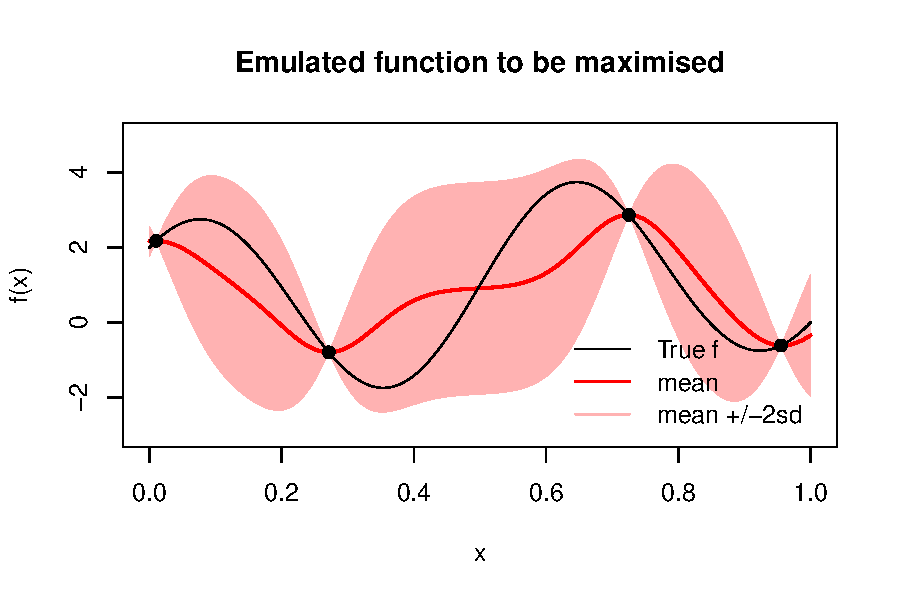
\includegraphics[width=\textwidth]{fig-optim/example-fn-to-maximise.pdf}
 \caption{A function, f(x), given by \cref{Eq:example-function}, to be optimised via BayesOpt with a corresponding emulator. The unknown function to be optimised is deterministic and given by the black line. The emulator mean is given by the solid red line and the translucent red region represents a $95\%$ probability band for $f(x)$. Plots of acquisition functions corresponding to this emulator are in \cref{Fig:acq-fns}.  \label{Fig:example-fn}}
\end{figure}
\begin{figure}[h]
 \centering
 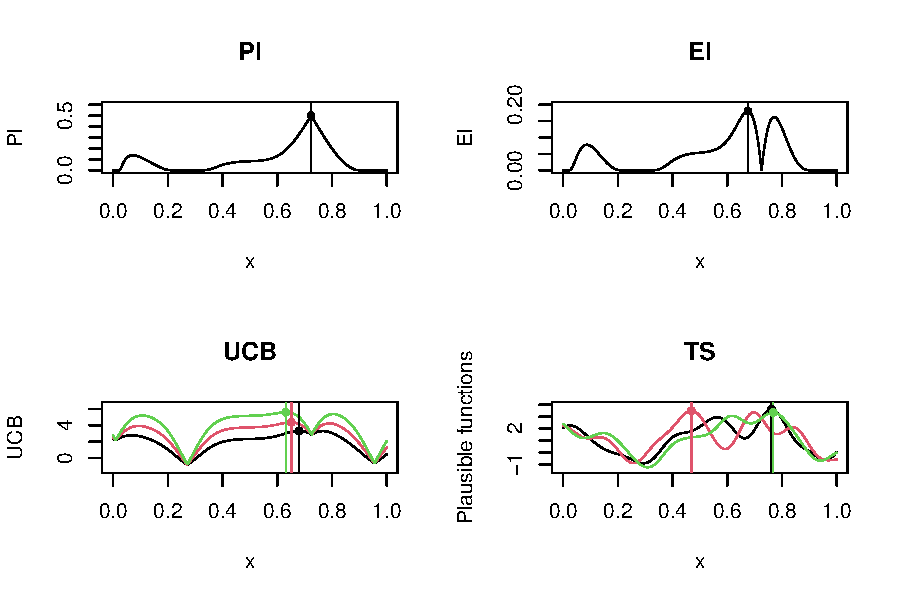
\includegraphics[width=0.8\textwidth]{fig-optim/example-acquisitions.pdf}
 \caption{Plots of acquisition functions for the function and emulator in \Cref{Fig:example-fn}. Vertical lines correspond to the maximiser of the acquisition function with the bullet being the the coordinates of the maximum. Three possible acquisition functions for UCB are shown corresponding to $\nu = 1, 2, 3$ and three random draws of $f(\cdot)$ are shown for TS. \label{Fig:acq-fns}}
\end{figure}
\subsection{Online GP updates for efficient BayesOpt}
BayesOpt is a sequential design problem. The emulator is updated as simulator runs arrive. GP prediction depends on the inversion of an $n \times n$ matrix. Matrix inversion is well known to be a slow (usually $\mathcal{O}(n^3)$) and numerically unstable operation.

By constructing a partition of $\Sigma_{n+1}$, the time $n+1$ precision matrix $\Omega_{n+1}$ can be expressed in terms of $\Omega_n = \Sigma_n^{-1}$ and the partitioned $\Sigma_{n+1}$. This partitioned representation is numerically stable and fast to compute. Consider the following partition of $\Sigma_{n+1}$
 \begin{equation}
 \Sigma_{n+1} = \begin{pmatrix}
         \Sigma_n + \lambda^2(X_n)I_n & c(\bx_{n+1}, X_n) \\
         c(\bx_{n+1}, X_n)^T & \sigma^2(\bx_{n+1}))
         \end{pmatrix}
 \end{equation}
 where $c(\bx_{n+1}, X_n)$ is the column vector of covariances between $\bx_{n+1}$ and the rows of $X_n$ and $\sigma^2(\bx_{n+1}) = \var\{ y(\bx_{n+1}) \}$. We then have
\begin{equation}
 \Omega_{n+1} = \begin{pmatrix}
         \Omega_n + k k^T /s & -k/s \\
         -k^T/s & 1/s
         \end{pmatrix} \label{Eq:omega-n1}
\end{equation}
where $k = \Omega_n c(\bx_{n+1}, X_n)$ is a length $n$ column vector and $s = \sigma^2(\bx_{n+1}) - c(\bx_{n+1}, X_n)^T k$ is a scalar quantity. This result can be confirmed by checking $\Sigma_{n+1} \Omega_{n+1} = \Omega_{n+1} \Sigma_{n+1} = I_{n + 1}$; see Section $3.4$ of \citet{Gentle2007} for the result and the Exercises of Section $3$ for a sketch proof. The only new information we need is $c(\bx_{n+1}, X)$ and $\lambda^2(\bx_{n+1})$, and if $\lambda^2(\bx)$ is assumed constant then it is already known. This amounts to calculating a length $n$ vector of covariances. Efficient updating via \Cref{Eq:omega-n1} works only if we condition on GP hyperparameters. This can be implemented if GP hyperparameters are only updated occasionally, or the results of a previous computer experiment may be used to estimate $\Theta$. We may also use the initialisation runs of BayesOpt to estimate $\Theta$. Sequential Monte Carlo can be used to perform efficient updates of a fully Bayesian posterior, under some appropriate assumptions \citep{Gramacy2011}.
\section{Decision making or decision support?}
We return to thinking about utility functions and the role of BayesOpt in making decisions. Once a BayesOpt scheme has been run, we have an emulator for the expected utility function, $U(\cdot)\mid \mathcal{D} \sim \mathcal{GP}(\cdot, \cdot)$ and an \textit{approximate} maximiser $\hat{\bx} = \argmax_{\bx \in X_n} \mu_n(\bx)$. In almost all applications of BayesOpt, it is common to stop here and report only $\hat{\bx}$. This is perhaps a symptom of the typical use case. A common use of BayesOpt is tuning hyperparameters of machine learning models where parameter uncertainty (decision uncertainty) is usually not regarded as important, or is difficult to incorporate \citep{Bergstra2011, Swersky2013, Kim2020}.

When making decisions for complex problems, one must possess great optimism to believe that the single, optimal decision can be uncovered when several necessary approximations to the truth have been forced upon us. It is myopic to report only the `best' decision. Many simplifications and approximations will have been used. Simulators are flawed representations of physical systems. The simulators will be a misrepresentation of the mathematical methods, for example, a numerical differential equation solver will be used. This will return a solution which is incorrect but close to the `true' answer implied by the underlying mathematics. Utility functions and prior beliefs will be misspecified to some degree and emulators provide a further, but necessary, approximation of the expected utility function. Therefore, $\hat{\bx}$ should not be taken as the ground truth; we should investigate other values of $\bx$ which lead to values of $U(\bx)$ which are `close' to $U(\hat{\bx})$. There is also an aspect of responsibility to consider. An analyst, who is junior to the decision maker, will typically be the individual tasked with running the BayesOpt scheme and reporting results, such as $\hat{\bx}$, to the decision maker, who has higher responsibility. If only $\hat{\bx}$ is reported, then one might ask what is the point of the decision maker? Another argument which favours decision support is the uncertainty about the utility function used. A comprehensive list of uncertainties in decision making is given by \citet{Dent2020}; some key aspects are:
\begin{itemize}
	\item[1.] Uncertainty associated to the simulator. Choice of input variables; choice of model fidelity; model discrepancy.
	\item[2.] Uncertainty about the simulator. When the simulator is expensive and/or stochastic, we rarely know the true output value or output distribution.
	\item[3.] Uncertainty about the utility function. The utility function is elicited and thus is prone to error induced by the elicitation process (e.g. biases or `random error' exhibited by the decision maker). This also includes the elicitation of appropriate decision attributes, as well as the parameters and functional form of the utility function.
\end{itemize}

In decision support, we should report more than just the (approximate) best solution to the problem. We should present multiple attractive solutions to the decision maker which take into account the above uncertainties.
\subsection{The Pareto front}
One approach to presenting multiple solutions, which is often utilised in engineering, is the Pareto front. The Pareto front is a collection of decisions which, in some sense, cannot be bettered. The notion of the Pareto front comes from multi-objective optimisation where the task is to maximise several single-attribute utility functions, $U_i(\bx)$, $i = 1, 2, \ldots, m$, that is, solve the following problem:
\begin{equation}
\text{maximise}\, U_1(\bx),  \text{maximise}\, U_2(\bx), \ldots, \text{maximise}\, U_m(\bx), \bx \in \calX.
\end{equation}
It is unlikely that the maximiser of $U_1(\bx)$ also maximises all the other $U_i(\bx)$. A trade-off is required. One example is the amount of time spent by a company constructing a wind farm. The decision maker can choose to employ more construction workers to improve the efficiency of the build, but if too many are employed at once or poorly managed, the build will be inefficient and costly. An analyst may calculate the monetary and time cost of each decision and report to the DM the decisions that form the \textit{Pareto front}. To define the Pareto front we first need to define a \textit{Pareto dominant} decision.

A decision $\bx \in \calX$ \textit{Pareto dominates} an alternative decision $\bx' \in \calX$ if, and only if, every attribute of $\bx$ is \textit{at least} as preferable as the corresponding attribute of $\bx'$ and at least one attribute of $\bx$ is preferred to the corresponding attribute of $\bx'$. That is
 \begin{equation*}
 \bx \succ_P \bx' \iff \,\forall \, i\, x_i \succeq x_i' \text{ and } \exists\, j \text{ such that } x_j \succ x'_j.
 \end{equation*}

Now, the Pareto front of $\cal{X}$, $PF(\calX)$, is the set of all decisions in $\calX$ which are not Pareto dominated:
 \begin{equation*}
 PF(\calX) = \left\{ \bx : \bx \in \calX \,\neg \exists\, \bx' \in \calX \text{ such that } \bx' \succ_p \bx \right\}.
 \end{equation*}
These definitions of Pareto dominant and Pareto front have been adapted from \citep{Roijers2017}. The Pareto front for the time and money example is given in \cref{Fig:pfront}. In this example, a set of possible decisions are plotted. It is cognitively complex for the DM to weigh up the relative merits of such a large set of decisions. It may also be computationally costly to investigate the consequences of each decision. Thus, only investigating the decisions which form the Pareto front simplifies the analysis.
\begin{figure}
 \centering
 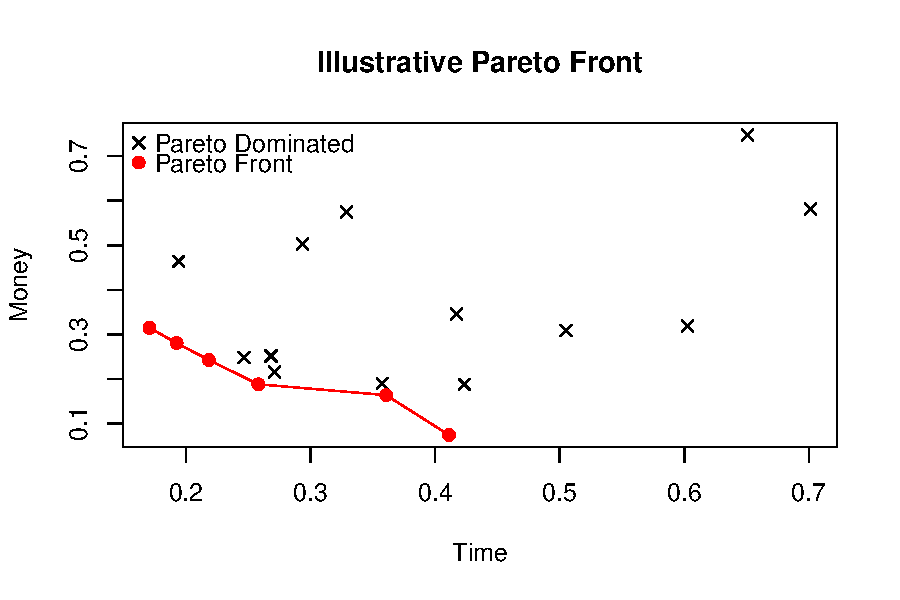
\includegraphics{fig-optim/pfront.pdf}
 \caption{An illustrative Pareto front for a collection of decisions. In this example, smaller values of the attributes Time and Money are preferred. The Pareto front is depicted by the red dots, which are connected by the red line, and consists of decisions for which no other decision offers smaller values of Time \textit{and} Money. The decisions which are Pareto Dominated are illustrated by black crosses. Any decision which is above/to the right of the Pareto front is a Pareto Dominated decision. \label{Fig:pfront}}
\end{figure}

A Pareto front is useful when we want to optimise multiple competing objectives, but it is not entirely clear how objectives compete. If the DM can settle on a utility function to express their preferences, the expected utility surface can (in theory) be maximised. When the utility function depends on the outputs of an expensive and stochastic simulator, maximisation in practice is incredibly difficult. BayesOpt methodology is well developed and can be used to find an approximate maximiser. However, there is only a relatively small amount of work on quantifying uncertainty about the optimal decision. A promising approach borrows ideas from the History Matching (HM) literature \citep{Lawson2016}.

\section{History matching}

HM is a procedure used to identify parameter settings of for a simulator which are consistent with observations from the corresponding physical system \citep{Craig1997, Domingo2020}. \correction{Suppose we have observed data $\by$, are able to specify a bounded domain $\bX \subset R^k$ of simulator inputs, and wish to infer parameters $\bx$ of a model,} statistical or otherwise, $y(\cdot)$.

The usual Bayesian and frequentist inference procedures aim to identify values of $\bx$ which best match $\yobs$, the observed data. This rests on the assumption that data $\yobs$ could be generated from the physical process which the simulator, $y(\cdot)$, aims to mimic. HM allows for many structures for $\yobs$. The nature of the work in this thesis means we only consider $\yobs \in \R$. HM addresses a more critical question than inference; are there \textit{any} values of $\bx \in \calX$ which are consistent with $\yobs$? As a corollary, if there are values of $\bx$ which are consistent with the observed data (allowing for various sources of uncertainty) then the HM toolkit allows us to find these values. These values are referred to as ``Not Ruled Out Yet'' (NROY). Let us consider an illustrative example. Consider the following simulator
\begin{equation}
 y(x) = 0.6 \sin (2 \pi x) + 2 \cos (3 \pi x) + \sin (4 \pi x) + 2x + \varepsilon^{*}, \, x \in [0,1] \label{Eq:hm-toy-fn}
\end{equation}
where $\varepsilon^{*} \sim \mathcal{N}(0,1)$ is an error term to account for all possible sources of uncertainty. Note that the deterministic part of \cref{Eq:hm-toy-fn} is identical to \cref{Eq:example-function}. We later decompose and discuss sources of error and uncertainty. This simulator is tractable and simple, we use this in place of a computationally expensive and complex simulator. Now suppose that we have observed the value $y = 2.5$ from the corresponding physical system. A frequentist could find the best input, $\hat{x}$, by minimising MSE or by specifying and maximising an appropriate likelihood function. Minimising MSE leads to one solution; $\hat{x} = 0.647$. The lack of uncertainty quantification about appropriate values of $\bx$ is a concern.

Uncertainty quantification is at the heart of Bayesian inference thus is a promising alternative. A Bayesian would specify their prior $x \sim \pi(x)$ then perform the usual Bayesian update. Since $y(\cdot)$ is thought to be complex, no conjugate form will exist thus a numerical scheme such as MCMC will be used, possibly assisted by a surrogate. Using Stan \citep{stan} and adopting the prior $x \sim \mathcal{U}(0,1)$ we constructed an MCMC sampler. The MCMC sampler aimed to obtain $10^4$ un-autocorrelated draws. With a burn in period of $10^8$ iterations, a further $10^8$ iterations were performed and thinned by a factor of $10^4$ to obtain $10^4$ draws from $\pi(x \mid y)$. Observing the histogram of posterior samples \correction{(right hand sub-figure of \cref{Fig:mcmc-chain}). The two} modes are centred on the two local maxima of $f(\bx)$, thus the posterior densities seem reasonable. However, the trace plot (left hand sub-figure of \cref{Fig:mcmc-chain}) appears to be `sticky' suggesting that inferences are not completely reliable and the lag $1$ autocorrelation is $0.919$. This is a common computational problem in Bayesian inference, despite our extensive thinning and burn-in periods.

Although we have experienced computational issues, which could be solved by running the Markov chain for a very long time, the Bayesian approach has an interpretation issue which is larger than any computational problem. What exactly does a prior, or posterior density, mean when trying to deduce appropriate decisions? Further, neither the likelihood nor posterior density are telling us which candidate decisions are sensible, given all biases and uncertainties. Allowing for biases and uncertainties within emulator assisted calibration frameworks is well understood \citep{Ohagan01, Goldstein2009} but if there is serious simulator-reality discrepancy, this may be due to a combination of misspecification of the underlying science, an error in the code or poor choice of tuning parameters in numerical solvers. Ultimately, this application of Bayesian inference does not tell us how to make sensible decisions under uncertainty.
\begin{figure}
 \centering
 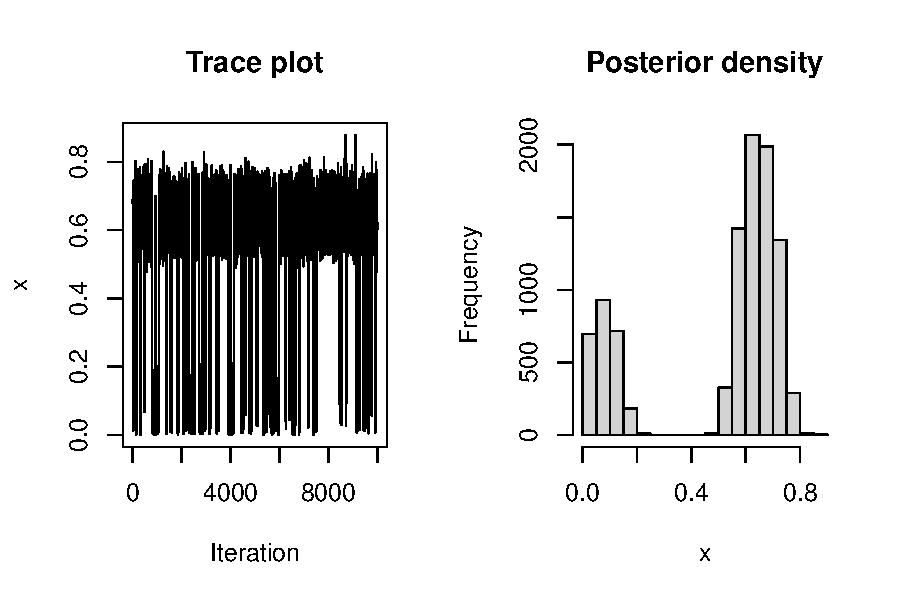
\includegraphics{fig-optim/trace-and-density.pdf}
 \caption{Trace plot (left) and posterior draws (right) from an MCMC sampler to infer appropriate value of $x$ in the illustrative example. \label{Fig:mcmc-chain}}
\end{figure}
\subsection{How can history matching help?}
HM finds appropriate simulator inputs based on how close $\E\{y(\bx)\}$ is to observed data $\yobs$, relative to all uncertainties that the DM is willing to consider. What we want to do is find decisions (parameters) which give an expected utility (simulator output) which is close to the maximum expected utility (observed data), whilst allowing for various uncertainties. These uncertainties may include the uncertainty in the utility function, which is characterised by the emulator, the uncertainty in the maximum expected utility and the uncertainty in the utility function and any simulators which feed into the utility function.

HM is based on a `best input' approach \citep{Ohagan01, williamson2013a}. Suppose that there exists a `best input' (or optimal decision) $\bx^{*}$ such that
\begin{equation}
 \yobs = y(\bx^{*}) + \varepsilon
\end{equation}
where $\varepsilon$ is an error term independent of $\bx^{*}$ and $y(\cdot)$. \correction{The goal of history matching is to find inputs that return outputs which are ``close'' to $y(\bx^{*})$, relative to all the uncertainties in the problem that we are willing to specify.} An implausibility measure, $I(\bx)$, is used to describe how appropriate $\bx$ is for data $\yobs$. Since most common emulation methods (GPs or Bayes linear methods) use expectations and variances for prediction and uncertainty quantification, implausibility measures often have the form in \cref{Eq:default-implausibility}.
\begin{equation}
 I(\bx) = \frac{| \yobs - \E \{y(\bx)\}|}{\sqrt{\var \{\yobs\} + \var\{y(\bx)\} + \var\{ \varepsilon_{\text{MD}} \} }} \label{Eq:default-implausibility}
\end{equation}
where $\varepsilon_{\text{MD}}$ is a mean-zero error-like term which accounts for model discrepancy. \correction{Structured model discrepancy has not been included in \cref{Eq:default-implausibility}. Where appropriate, structured model discrepancy could be removed via the numerator of the given implausibility function.} This proposed implausibility measure is well suited to simulators with a single output. Multivariate implausibility measures have also been proposed and are usually based on the Mahalanobis distance or by specifying an implausibility function for each simulator output, $I_j(\bx)$, and taking $I(\bx) = \max_j I_j(\bx)$. The Mahalanobis distance deems an input as implausible if, jointly, the set of outputs is unusual. The maximum implausibility approach deems an input as implausible if at least one of the outputs is unusual. Both types of multivariate implausibility have been shown be effective in practical examples \citep{Vernon2010,Williamson2017}.

We consider $\bx$ to be an appropriate value, termed `not implausible', when $I(\bx) < I_0$. Often $I_0 = 3$. This value stems directly from Pukelsheim's $3\sigma$ rule \citep{Pukelsheim1994}. The $3\sigma$ rule states that, if $Z$ follows a unimodal, continuous distribution with $\E(Z) = \mu < \infty$ and $\var(Z) = \sigma^2 < \infty$ then
\begin{equation}
 \p \left( | Z-\mu | \geq 3\sigma \right) < 0.05. \label{Eq:pukelsheim}
\end{equation}
Thus using the $3\sigma$ rule means we incorrectly rule out a value of $\bx$ no more than $5\%$ of the time. Pukelsheim actually proved a slightly tighter bound than this, but $\p ( |Z - \mu| \geq 3\sigma ) \leq 4/81 \approx 0.04938$ fails to roll off the tongue so smoothly. If we are to make distributional assumptions about $f(\cdot)$ and $\yobs$, we can make this bound tighter. In the Gaussian case, it is well known that approximately $5\%$ of values lie outside of $\mu \pm 2 \sigma$ and fewer than $1\%$ of values lie outside of $\mu \pm 3\sigma$. Using the $3\sigma$ rule even when probabalistic assumptions are made about $y(\cdot)$ may offer some robustness to misspecification of such assumptions. This is not the only form of implausibility function; any function which suitably measures the difference between the data and the simulator output, relative to all sources of uncertainty is a candidate implausibility function. For example, \citet{Wang2018} use $p$-values to quantify implausibility.

Returning to \cref{Eq:default-implausibility}; $\E\{y(\bx)\}$ and $\var \{ y(\bx) \} $ are critical to many applications of HM. These expectations and variances may be the true mean and variance of $y(\bx)$ when the moments are known. If $y(\bx)$ is intractable, then these can be replaced with the posterior (or adjusted) mean and variance of $y(\bx)$; the inclusion of emulators into the HM framework is natural.

A graphical implementation of HM is given in \cref{Fig:example-hm-graph}. Here we have emulated $y(\cdot)$ and assumed that $\var\{\varepsilon\} = 0.75$, $\var\{\yobs\} = 0.25$ and further assumed $\var\{\varepsilon_{\text{MD}} \} = 0$ (i.e. the simulator is a perfect representation of the physical system). We see that using a cutoff of $3$, some regions of the input space are incompatible with the data. The green regions of the right hand plot of \cref{Fig:example-hm-graph} represent the (wave $1$) NROY space. A mathematical description of this space is
\begin{equation}
 \calX_{\text{NROY}} = \{ x \in \calX : I(x) < I_0 \}
\end{equation}
where we have chosen $I_0 = 3$, justified by Pukelsheim's $3\sigma$ rule.
\begin{figure}
	\centering
	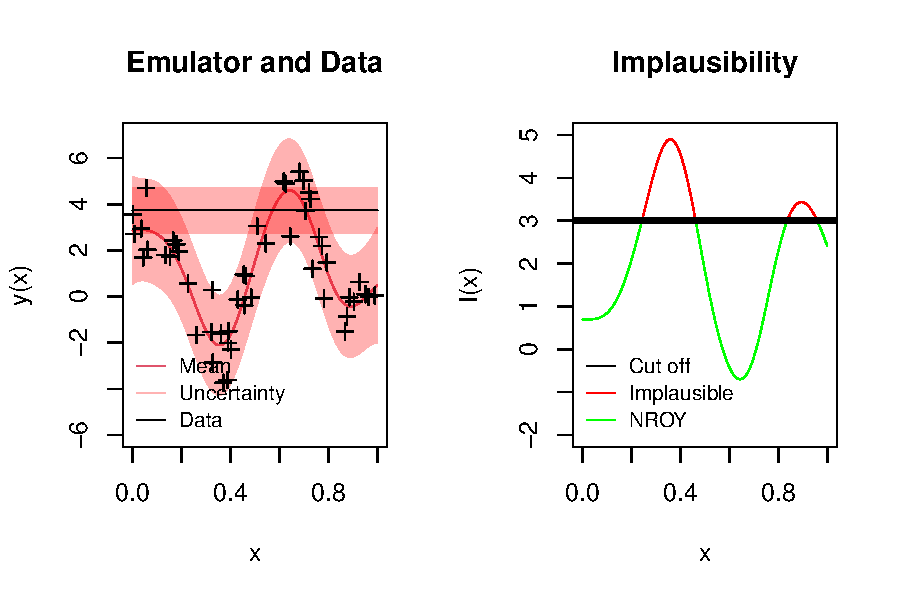
\includegraphics{fig-optim/implaus1.pdf}
	\caption{Illustrative HM procedure for the simulator given in \cref{Eq:hm-toy-fn}. The left hand plot shows an emulator, whose training data are the black `$+$' symbols and $\yobs$ is given as the black horizontal line. The emulator mean has an approximately sinusoidal shape, with pink uncertainty bands about the observed data as well as the emulator. The right hand plot shows the corresponding implausibility function which is colour coded. The red parts of the function ($I(x) \geq 3$) correspond to implausible values of $x$ whilst green regions ($I(x) < 3$) correspond to NROY regions. The black line is the cut off; $I(x) = 3$. \label{Fig:example-hm-graph}
}
\end{figure}
This first wave of HM has led to $34.2\%$ of the original space being ruled out as inconsistent with $\yobs$. HM is well suited to sequential analysis. We can construct new emulators in the NROY space. These new emulators should have reduced uncertainty about them because emulators typically exhibit reduced uncertainty in regions where simulator runs are dense. Since this is an illustrative example, we construct one emulator over the entire NROY space, which is the union of three distinct sub-spaces. When the NROY space is a union of two, or more, disjoint subsets of $[0,1]$, it may be advantageous to construct an emulator on each disjoint subset. This will result in faster matrix calculations. Matrix multiplication is typically $\mathcal{O}(n^2)$ and inversion is typically $\mathcal{O}(n^3)$, now $a(n^k) < (an)^k$ for $a, k > 1$ thus if we have $a$ distinct regions, emulation will be faster if we construct distinct emulators over each distinct region. If the function is non-stationary (which is often the case, but computationally complex to implement over a non-disjoint spaces), allowing for different parameters in different regions of the input space should produce emulators which are a better representation of $y(\cdot)$ \citep{Gramacy2008}.

A second wave of runs was produced. This second wave of runs and emulation allowed us to rule out a further $13.4\%$ of the remaining space. The revised NROY space is now $57\%$ of the original space. We see that each of the two NROY regions in \cref{Fig:example-hm-graph2} corresponds to a neighbourhood around each of the two local modes of $f(\bx)$ since $\yobs = \max f(x)$.
\begin{figure}
 \centering
 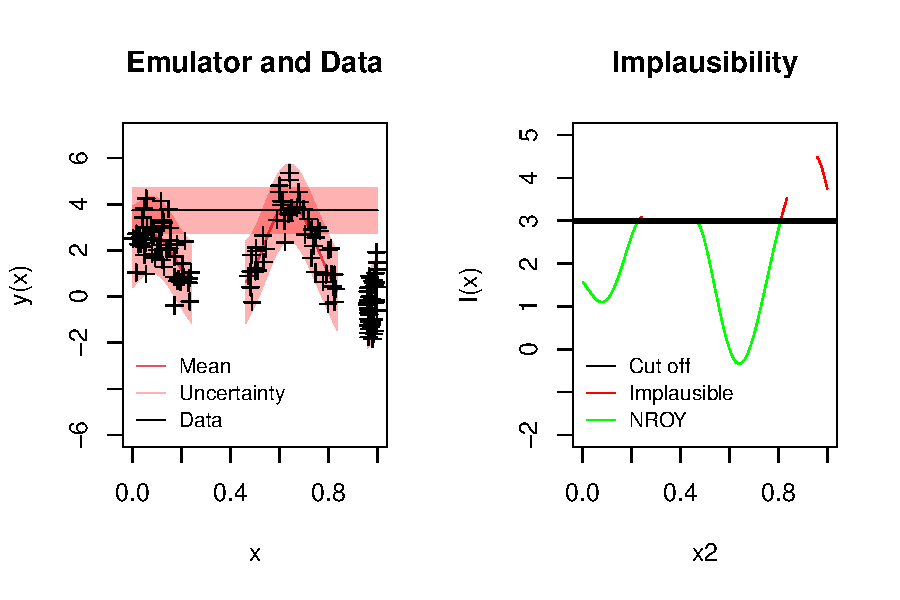
\includegraphics{fig-optim/implaus2.pdf}
 \caption{Illustrative wave $2$ HM procedure for the simulator given in \cref{Eq:hm-toy-fn}. The left hand plot shows an emulator, whose training data are the black `$+$' symbols; $\yobs$ is given as the black horizontal line. The emulator has an approximately sinusoidal shape, with pink uncertainty bands about the observed data as well as the emulator. The right hand plot shows the corresponding implausibility function which is colour coded. The red parts of the function ($I(x) \geq 3$) correspond to implausible values of $x$ whilst green regions ($I(x) < 3$) correspond to NROY regions. The black line is the cut off; $I(x) = 3$. Gaps in both graphs represent the space ruled out after the first wave of HM. These are automatically ruled out at this stage, thus are not considered. }
 \label{Fig:example-hm-graph2}
\end{figure}
 In this instance, we generated inputs uniformly from each sub-region of the NROY space and allowed an equal number of samples in each sub-region. Because this is a one dimensional problem, it is easy to identify the NROY space by inspection. For higher dimensional problems, the only way to identify the NROY region is by evaluation of the implausibility function \citep{Williamson2013}. This is due to the black-box nature of emulators. When multiple waves of emulators have been produced, we may have to evaluate many implausibility functions. If we have performed $k$ waves of emulation, the wave $k+1$ space is given by
\begin{equation}
 \calX_{k+1} = \{ \bx \in \calX_k : I^{k}(\bx) < I^k_0 \}
\end{equation}
where $I^k(\cdot)$ is the wave $k$ implausibility function and $I^k_0$ is the wave $k$ cut off. Note that $k$ here is a superscript and not an exponent. This recursive definition means we \textit{might not} have to evaluate all $k$ implausibility functions to know if $\bx \notin \calX_{k+1}$. Since this requires multiple matrix calculations, this can become computationally costly. To speed up the computation, we should start by evaluating $I^1(\bx)$, then $I^2(\bx)$ and so on. If any $I^j(\bx) \geq I^j_0$, then we should stop evaluation of further implausibility functions since $\bx$ has been ruled out.

Adapting HM to optimisation is a promising tactic when an analyst wants to perform decision support. HM provides a solution to the problem of constructing an interpretable set of decisions which are acceptable, whilst allowing for all relevant uncertainties and biases. The interpretation here is that these decisions are within a given tolerance of the current best decision. This also allows for uncertainty about the best decision seen so far, as, when $y(\cdot)$ is stochastic, there will typically be uncertainty about $U(\bx)$. The analyst can then report $\calX_{k+1}$ to the decision maker; it represents a set of decisions which are not clearly worse than the reported optimal decision, given all the uncertainties considered.
\subsection{Drawbacks of HM}
\correction{HM is not a perfect approach, there are potential drawbacks that we should be aware of.}

\correction{The first potential drawback is that, once a point has been deemed NROY, it is NROY for all future waves. This means, if we were to rule out $\bx^{*}$, no future waves would contain the optimal decision, or best input, as appropriate.}

\correction{Another potential drawback is that, at the number of waves grows, we are increasingly likely to rule out good points. The error rate for a history matching is often defined at the wave-level. Over multiple waves of HM, the proportion of incorrectly ruled out points is compounded. For a large number of waves, this means we are in danger of ruling out large regions of the input space that leads to good decisions, or is compatible with observed data.}

\correction{A third drawback is that characterising the NROY space is achieved by random sampling. This means, it is not possible to fully understand the NROY region. For example, if a sampling scheme used to describe the NROY space missed a disconnected region of the NROY space, we might not know. In practice it is hard to tell if disconnected regions exist, and even harder to tell if we have captured all of them.}

\subsection{HM for decision support}
When using HM techniques for optimisation or decision support, the implausibility measure used must be different from \cref{Eq:default-implausibility}. This is because, (i) we have not observed data from a physical system and (ii) the modulus operation in the numerator will cause problems if the emulator predicts a value larger than the current largest value. Recall that the goal is to maximise $f(\bx)$, thus, within decision support, authors typically use an implausibility measure of the form
\begin{equation}
 I(\bx) = \frac{y^* - \E \{f(\bx)\} }{\sqrt{ \var\{y^*\} + \var\{f(\bx)\} + \var\{\varepsilon_{\text{MD}}\}}}.
\end{equation}
\citet{Owen2020} uses this implausibility function but set $I(\bx) = 0$ whenever $\E\{ f(\bx) \} > y^{*} $. \citet{Baker2020c} retains the exact value of $I(\bx)$ to communicate which decisions are much likely to be better than our reference value. If $I(\bx) \leq -3$, then $\bx$ is `ruled in' as a good candidate decision, since it is much larger than the reference value $y^{*}$. The $\bx$ satisfying $I(\bx) \geq 3$ are ruled out, as is standard. Then, the next wave is constructed in the range for which $|I(\bx)| < 3$ to allow the analyst to explore the decisions for which it is not clear if they are acceptable or not.
\begin{figure}
 \centering
 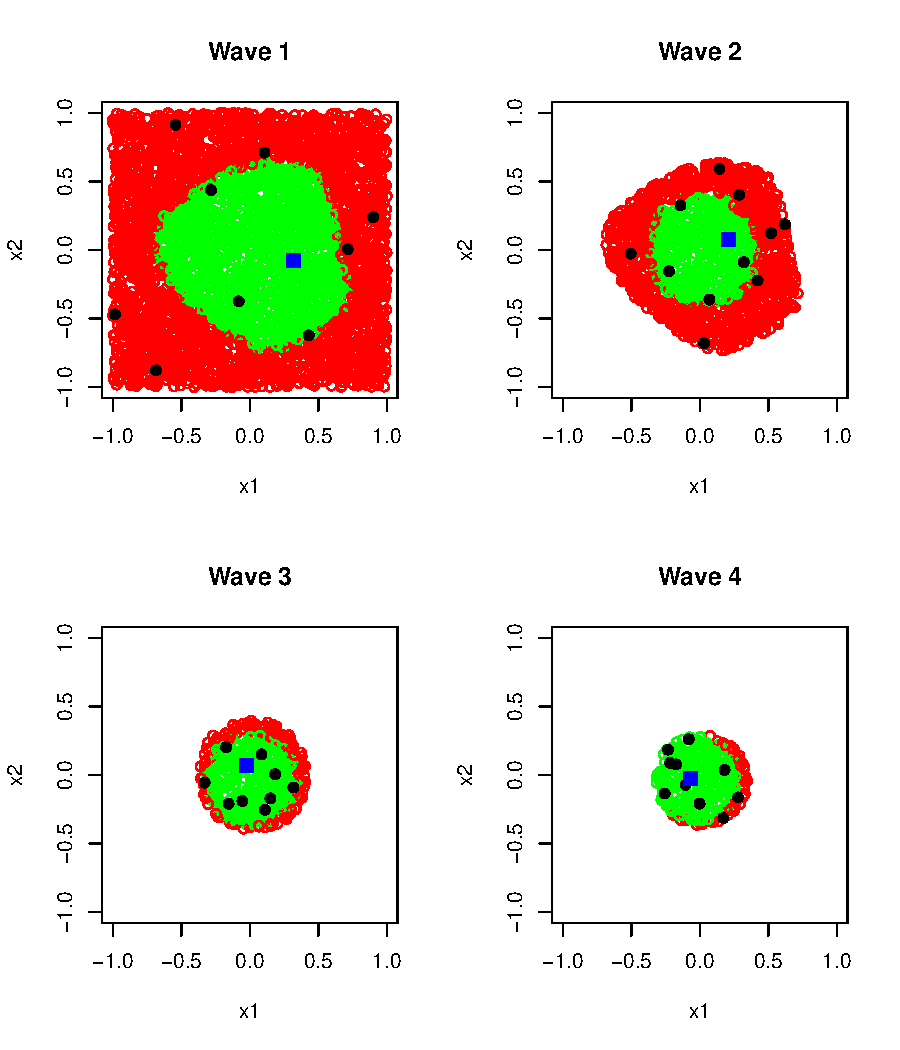
\includegraphics{fig-optim/quad-optim.pdf}
 \caption{An illustrative example of using HM inspired techniques to construct a set of good decisions under uncertainty. The circles are a large set of candidate decisions; red circles denote decisions that have just been ruled out ($I^k(\bx) \geq 3$) whereas green decisions are those which are NROY ($I^k(\bx) < 3$). Black dots are design points for the wave $k$ emulator with the blue square being the design point with largest expected utility at wave $k$. \label{fig:quad-optim}}
\end{figure}
An illustrative example of iterative HM inspired decision support is given in \cref{fig:quad-optim}. This method of fitting a sequence of emulators (not to be confused with sequential design\footnote{It could be argued that iterative refocussing is a batch-sequential design where the size of the batches is much larger than the number of batches.} like BayesOpt or ALM) is sometimes termed ``iterative refocussing'' as the NROY space focuses in on a smaller region after each wave of emulation/HM \citep{Williamson2017, Volodina2021}. Here we are trying to optimise a utility function $U(\bx) = 2 - x_1^2 - x^2_2$ but the observations are noisy; $y(\bx) \sim \mathcal{N}(U(\bx), 0.1^2)$. We specified a model discrepancy variance of $\var\{\varepsilon_{\text{MD}}\} = 10^{-6}$.

Each wave of emulation allows us to concentrate simulator runs on regions of the input/decision space which typically produce larger values of $U(\bx)$. This allows for improved decision making because the expected utility values are usually increasing. Also the emulators become more accurate within the NROY region as it shrinks; this means that the emulator mean response at later waves typically becomes a more accurate representation of $U(\bx)$. Although the NROY volume shrinks, due to the reduction in $\var\{f(\bx)\}$, $\var\{\varepsilon_{\text{MD}}\}$ is a limiting factor in the reduction of the NROY space, and to some extent the uncertainty about the optimal decision, $\var\{U^{*}\}$ will also be a limiting factor (in principle, this will shrink to $0$ as the number of runs grows, but runs are expensive thus limited). This means that, eventually, iterative refocussing will lead to diminishing returns. We have illustrated the diminishing returns in \cref{fig:nroy-numbers}; the volumes shown in these two sub-figures correspond to the NROY volumes in each sub-figure of \cref{fig:quad-optim}. We see that the size of the NROY volume decreases drastically in the first two waves of emulation, but the latter two waves lead to more modest reductions in the number of NROY decisions. This is explained by $\var\{ f(\bx) \}$ reaching a small value. After each wave of emulation, the average value of $\var\{f(\bx)\}$ within the NROY regions $\calX_2$ through to $\calX_5$ is $(1.79, 0.35, 0.087, 0.14)\times 10^{-2}$. After each of the first three waves of emulation, the average variance typically decreases by a significant fraction. The final wave leads to a slight increase in the average variance. This is likely a random artefact of the sample, the final average variance is of similar size to the third, and the reduction in the NROY volume is small, which suggests we should terminate the HM procedure.
\begin{figure}
 \centering
 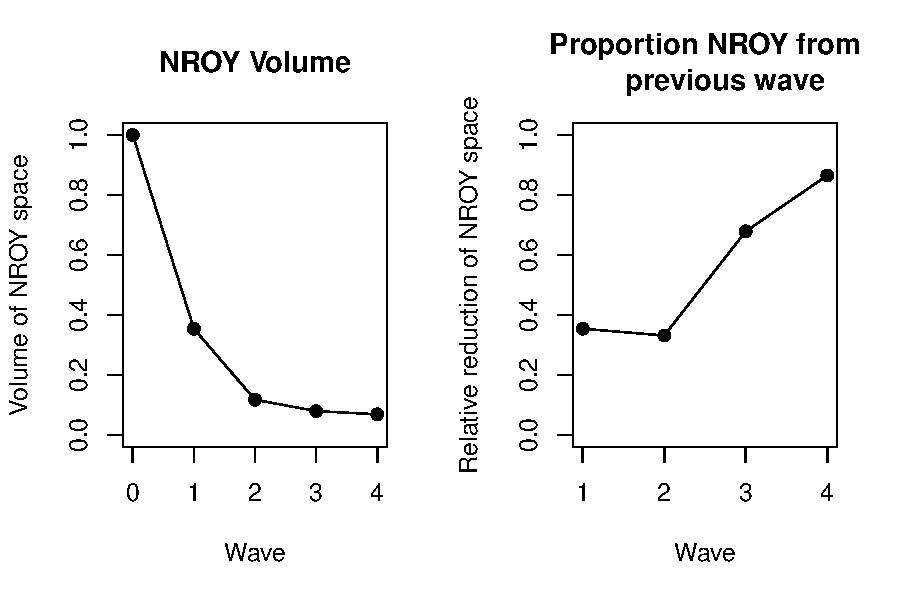
\includegraphics{fig-optim/nroy-reduction.pdf}
 \caption{Graphs depicting how the volume of the NROY region shrinks as the number of waves increases. The left hand plot shows the ratio $|\calX_{k+1}|/|\calX|$ which is the proportion of NROY decisions remaining after $k$ waves of emulation and HM; we see the first two waves lead to larger reductions in the NROY volume than the latter waves. The final wave of emulation leaves us with just $7\%$ of the original space as NROY. The right hand plot shows $|\calX_{k+1}|/|\calX_k|$, that is, the proportion of decisions that are NROY after wave $k$ that are also NROY at wave $k+1$. The right hand plot shows that the second wave was, in some sense, slightly more effective than the first wave. However the $4$th wave of emulation only ruled out $13\%$ of points in $\calX_4$, which is small thus the HM procedure was terminated. The $0$th `wave' denotes all the initial volume (prior to emulation/HM).\label{fig:nroy-numbers}}
\end{figure}

\subsubsection{How does HM address exploration versus exploitation?}

In BayesOpt, we can analyse the exploration-exploitation trade-off by studying acquisition functions. For HM inspired techniques we take a less technical approach to arguing that HM satisfies the trade-off.

During each wave of HM, we construct a design in $\calX_{k+1}$ which is, in part, based on an implausibility measure. The measure is of the form
\begin{equation}
 I_{k+1}(\bx) = \frac{y^{*} - m^{*}(\bx)}{ \sqrt{v^{*}(\bx) + k} }
\end{equation}
where $k$ represents other sources of uncertainty such as model discrepancy. Clearly, if $m^{*}(\bx)$ is large, then $I_{k+1}(\bx)$ will be small. Similarly, if $v^{*}(\bx)$ is large, $I_{k+1}(\bx)$ will also be small. We retain $\bx$ for future study when $I_{k+1}(\bx)$ is small. Exploitation is achieved in two ways; firstly, by reversing the previous argument, when $m^{*}(\bx)$ and $v^{*}(\bx)$ are both small, we will not retain $\bx$ at the next wave. This effect applies to previous waves also. We are only considering points which have previously been identified as promising or uncertain, thus we are exploiting knowledge from previous waves of emulation.

Some additional exploration, which is not present in BayesOpt, can be achieved via $k$. Large values of $k$, corresponding to larger model discrepancy and/or other sources of uncertainty, typically lead to larger NROY spaces. This means we consider a larger volume of decisions at later waves. Further, since the HM inspired approach reports uncertainty about the best decision seen so far, once we have terminated the HM procedure there is more exploration to be done. The decision maker themselves must consider decisions which are still NROY to settle on a final decision.


\subsection{Wave $k>1$ designs}

A design is required for each wave of emulation. In wave $1$, LH sampling is the usual approach due to the space filling properties of LHs. For waves $2$ and beyond, the design space is characterised by the implausibility measure. The resulting NROY space has no obvious form when expressed as a function of $\bx$, this is seen in \cref{fig:quad-optim}. Although not a rigorous term, `blob shaped' would be a reasonable description. Ultimately the NROY space depends on the posterior mean and variance given by an emulator. Thus the only way to know if $\bx$ is ruled out after $k$ waves of emulation is to evaluate $I^k(\bx)$. This often leads to NROY regions with unusual shapes \citep{Garbunoinigo2020}. As a result of the NROY space being defined in a black-box manner, design for waves $k>1$ can be a challenging task.

The simplest approach to (uniform) design for a wave $k+1$ emulator is rejection sampling. Usually, a large LH is constructed over the original input space and then the points which are NROY after $k$ waves are retained for the wave $k+1$ emulator \citep{Vernon2010}. This approach is reasonably efficient when the NROY space is a relatively large fraction of the original space (say, more than $1\%$ of the original space). When the NROY space is a small fraction of the original space, the approach becomes very expensive. If, after $k$ waves of emulation, $|\calX_{k+1}| = p_k|\calX|$ then if we want $N$ NROY samples we would expect a LH of size $N/p_k$ to give us $N$ NROY samples. This problem is harder in higher dimensional spaces due to the curse of dimensionality and also more computationally expensive when we use non-random LHs (for example, maximin LHs). Another problem with this approach is that it returns a design of a random size. If we know we can perform no more than $N$ runs of the simulator at each wave, we would usually want to perform exactly $N$ runs.

There are promising alternatives to rejection sampling, based on other Monte Carlo schemes. The Monte Carlo schemes all take the same view on the problem. Sampling uniformly from $\calX_{k+1}$ is mathematically equivalent to sampling from the following density
\begin{equation}
 \pi_{k+1}(\bx; I_0) \propto \begin{cases}
  1, & I^k(\bx) < I_0\\
  0, & I^k(\bx) \geq I_0
 \end{cases}.
\end{equation}
 \citet{Williamson2013} use evolutionary Monte Carlo (EMC) and \citet{Drovandi2021} use sequential Monte Carlo (SMC) to construct NROY designs for which the the NROY space is a tiny subset of $\calX$. Another promising approach, which is conceptually much simpler than the EMC and SMC approaches, is slice sampling. Within the HM context, this was first used by \citet{Andrianakis2017a} and the slice sampler for iterative refocussing is simpler than the standard slice sampling algorithm since the density is constant within $\calX_{k+1}$ \citep{Neal2003}.

\subsection{Slice sampling for NROY regions}

We now provide some details of the slice sampling algorithm introduced by \citet{Neal2003}, which is given in \cref{alg:neal-slice} and compare this to the sampler used by \citet{Andrianakis2017a}, which we describe in \cref{alg:nroy-slice}. We will aim to sample from a density $\pi(\bx)$ which is only known up to proportionality; $\pi(\bx) = k \varphi(\bx)$ where $k^{-1} = \int \varphi(\bx) \, \diff \bx$ is an intractable normalisation constant. A version of the algorithm proposed by \citet{Neal2003} is given in \cref{alg:neal-slice}, and a corresponding illustration for a univariate example is given in \cref{Fig:slice-diagram}, where $\varphi(\bx)$ is a linear combination of three univariate Normal densities. The vertical blue line denotes our initial sample, $x_0$, and the horizontal blue line denotes $\varphi(x_0)$. The horizontal red line represents the horizontal slice $y_0 \sim \mathcal{U}(0, \varphi(x_0))$ and then the dashed red lines illustrate the sample space for the next sample, $x_1$. A uniform sample along the $x$ axis where red dashed lines are present gives us our next draw from $\pi(x)$. Slice sampling is a powerful sampling technique because we only need to be able to (i) sample uniformly and (ii) solve equations (construct the horizontal slice). The equation solving aspect can be challenging. Our illustrative, one-dimensional example had four roots to find. In a complex high dimensional problem, we may not know how many roots exist.

The standard slice sampler (\cref{alg:neal-slice}) differs somewhat from the slice sampler for NROY regions (\cref{alg:nroy-slice}). A similarity between the two is that they are both component wise; each element of $\bx$ is updated one-by-one. Some steps in the standard slice sampler are not required for generating samples from the NROY region. The first difference is that in \cref{alg:nroy-slice} we do not calculate $\varphi(\bx_0) = \mathbb{I}(\bx_0)$ because we know it is $1$. Secondly, we do not sample $y_0 \sim \mathcal{U}(0, \varphi(\bx_0))$ because $\varphi(\bx)$ is either $0$ or $1$. Any NROY sample satisfies $\mathbb{I}(\bx \in \calX_{k+1}) = 1$, therefore $y_0=1$ in all cases. This bypasses the tricky root finding problem.

Slice sampling, as in \cref{alg:nroy-slice}, allows us to update the $i$th input. The slice sampling can be made drastically more efficient by changing the limits of the uniform proposal. If it is known that $\calX_{k+1} \subseteq [l_1, r_1] \times [l_2, r_2] \times \ldots [l_m, r_m]$ then we can replace the $\mathcal{U}(0,1)$ random sample with a $\mathcal{U}(l_i, r_i)$ sample, where $0 \leq l_i < r_i \leq 1$. This efficiency gain may come at a cost: if an $l_i$ or $r_i$ are misspecified, we would neglect parts of the NROY space. For input $i$, suppose $l_i$ is chosen to be too large, then any $\bx \in \calX_{k+1}$ such that $x_i < l_i$ would never be sampled.
\begin{figure}[h]
 \centering
 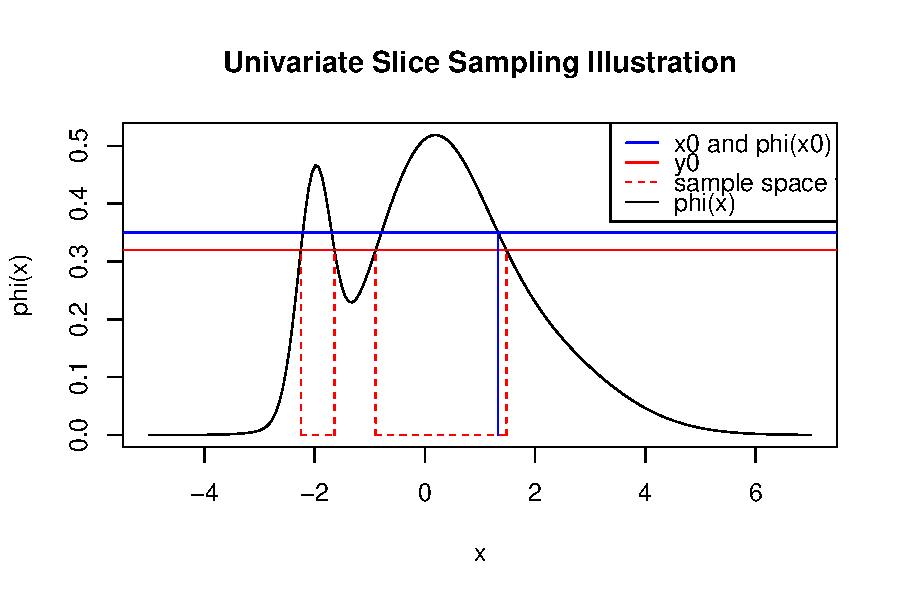
\includegraphics{fig-optim/slice-diagram.pdf}
 \caption{An illustration of how to sample $x_1 \sim \pi(x)$ given a draw $x_0 \sim \pi(x)$ when the only information we have about $\pi(x)$ is that $\pi(x) \propto \varphi(x)$. The black curve represents $\varphi(x)$, the vertical blue line represents $x_0$, the initial sample and the horizontal blue line represents $\varphi(x_0)$. The horizontal solid red line represents $y_0 \sim \mathcal{U}(0, \varphi(x_0))$. The dashed red lines denote the space in which $x_1$ is uniformly sampled from to obtain a new draw from $\pi(x)$.\label{Fig:slice-diagram}}
\end{figure}
\begin{algorithm}[h]
\caption{A single iteration of a generic, component-wise slice sampler, based upon the slice sampler presented by \citet{Neal2003}. \label{alg:neal-slice}}
\begin{algorithmic}
\Require A density known up to proportionality $\pi(\bx) \propto \varphi(\bx)$, an initial sample $\bx_0 \sim \pi(\bx)$ where $\bx_0$ is an $m$ dimensional parameter vector.
\State $\bx_1 \gets \bx_0$
\For{$i = 1$, $2$, $\ldots$, $m$}
 \State $\varphi_0 \gets \phi(\bx_0)$ and sample $y_0 \sim \mathcal{U}(0, \phi_0)$
 \State Find the set $\tilde{\calX} = \{x_i : \varphi(x_i, \bx_{-i}) \geq y_0 \}$
 \State Draw $\tilde{x}_i \sim \mathcal{U}(\tilde{\calX})$\Comment{Sample uniformly from $x \in \tilde{\calX}$}
 \State Set $x_{1,i} \gets \tilde{x}_i$ \Comment{Update the $i$th component of $x_0$}
\EndFor
\State Return, $\bx_1$, the new sample from $\pi(\bx)$.
\end{algorithmic}
\end{algorithm}
\begin{algorithm}[h]
\caption{A single iteration of a component-wise slice sampler used for sampling from NROY regions, based upon the slice sampler presented by \citet{Andrianakis2017a}. \label{alg:nroy-slice}}
\begin{algorithmic}
\Require An indicator function $\mathbb{I}(\bx \in \calX_{k+1})$ for identifying inputs which are NROY, an initial NROY point $\bx_0 \in \calX_{k+1} \subseteq [0,1]^m$ where $\bx_0$ is an $m$ dimensional parameter vector.
\State $\bx^{*} \gets \bx_0$
\For{$i = 1$, $2$, $\ldots$, $m$}
 \State $I^{*} \gets 0$ \Comment{Initialise an indicator variable}
 \While{$I^* \neq 1$}
  \State Draw $x_i \sim \mathcal{U}(0,1)$ \Comment{Change the $i$th input}
  \State $x^{*}_i \gets x_i$
  \State $I^{*} \gets \mathbb{I}(\bx^{*} \in \calX_{k+1})$ \Comment{Evaluate the implausibility measure at the new input}
 \EndWhile
 \State $\bx_1 \gets \bx^{*}$ \Comment{Update the $i$th component of $\bx_0$}
\EndFor
\State Return, $x_1$, the new sample from $\pi(\bx)$.
\end{algorithmic}
\end{algorithm}
\correction{
However, \cref{alg:nroy-slice} has an issue: in general, it is not \textit{ergodic}. That is, it may not be possible to fully explore $\calX_{k+1}$ with a single run of the algorithm. This can be amended by repeating the algorithm for many initial points $\bx_0$ which are randomly chosen (for example, by sampling uniformly in $[0,1]^m$ until we find an NROY point).}

We formalise this in \cref{alg:ergodic-slice}.

\begin{algorithm}[h]
\caption{An ergodic variant of \cref{alg:nroy-slice}. \label{alg:ergodic-slice}}
\begin{algorithmic}
\Require An indicator function $\mathbb{I}(\bx \in \calX_{k+1})$, a number of replications, $R$, a required number of samples, $n =  n' \times R$, and a function $\texttt{slice\_sampler\_one\_step}(\mathbb{I}(\bx \in \calX_{k+1}), \bx_0)$ which takes an implausibility function, $\mathbb{I}(\bx \in \calX_{k+1})$ and an NROY point, $\bx_0$ and returns a new NROY point.

\For{$r = 1, 2, \ldots, R$}
  \State {$I_r \gets 0$}
  \State Initialise a matrix $X_r$ with $m$ columns and $n'$ rows
  \While{$I_r \neq 1$}
    \State $\bx_{1, r} \gets \mathcal{U}([0, 1]^m)$
    \State $I_r \gets \mathbb{I}(\bx{1, r} \in \calX_{k+1})$
  \EndWhile
  \For{$i = 2, 3, \ldots, n'$}
  \State $\bx_{i, r} \gets \texttt{slice\_sampler\_one\_step}(\mathbb{I}(\bx \in \calX_{k+1}), \bx_{i-1, r})$
\EndFor
\EndFor
\State Collect all $X_r$ into a single matrix $X$, with $m$ columns and $n$ rows.
\State Return $X$, the collection of NROY samples.
%\Return $X$, a sample of $n$ NROy points.
\end{algorithmic}
\end{algorithm}

\section{Discussion}

This chapter has reviewed methods for decision making under uncertainty to prepare us for the next chapter, in which we solve a decision problem using some of the illustrated techniques. We began by considering decision making as an optimisation problem. We discussed that although mathematically well defined, decision making is a difficult task. The difficulty of the problem is increased when we have limited understanding of $U(\bx)$ due to the stochastic, expensive and gradient-free nature of many simulators.

We discussed various optimisation methods, then settled on Bayesian Optimisation as being an efficient and effective approach to \textit{decision making} with complex models. We discussed various acquisitions functions and presented decision theoretic justifications for each acquisition function, where relevant. A consequence of using BayesOpt for decision making is that it makes decisions on behalf of the DM, which poses questions about \emph{who} is making decisions. We argue that viewing complex, ill-defined problems as those possessing a single, optimal solution is myopic. An appropriate approach to addressing these concerns is to use \textit{decision support} to simplify, but not solve, the problem for the decision maker. We discussed the idea of a Pareto front as a decision support tool, however, we are working within a regime where a utility function has been established but is expensive to evaluate. We therefore treat $U(\bx)$ as an unknown function which is optimised under multiple sources of uncertainty. These may include the uncertainty induced by the expensive nature of the utility function, any stochasticity present in simulations, uncertainty about model parameters which are not decision parameters as well as the uncertainty about the elicited utility function.

Therefore, we settled on using HM inspired techniques to iteratively hone in on a set of feasible solutions, called the NROY space. These decisions are a set of solutions, which, given all relevant sources of uncertainty, are not worse than the best decision we have found so far. We briefly discussed some approaches to iterative construction of emulators, and in particular discussed some approaches to the wave $k>1$ design problem. Monte Carlo methods, commonly used to perform Bayesian inference, offered a promising solution to constructing uniform designs across the NROY space. In particular, we advocate for slice sampling as it strikes a good balance of conceptual simplicity, computational simplicity and effective results. The only mechanism we need in addition to the implausibility function is a uniform sampling scheme, and all major scientific computing libraries allow for uniform sampling.

Empirical evidence tells us that these are typically much more efficient than rejection sampling when $|\calX_k|$ is a tiny fraction of $|\calX|$. However, we did not discuss how to get the optimum `reference' value, which is central to the HM inspired approach. In the next chapter, we explore this further and employ a slice sampling approach to construct a set of feasible decisions.
\end{chapter}
